\setcounter{chapter}{1}
\chapter{Modèles de Drude et de Sommerfeld}
\section{Modèle de Drude}
	\subsection{Modèle de Drude pour les métaux}
	Malgré que le modèle de Drude soit ancien (1900) il est toujours utilisé 
	aujourd'hui. A cette époque, l'électron n'a été mis en évidence que depuis 
	trois ans : la physique quantique n'est pas encore connue mais les équations 
	de Maxwell, elles, le sont bien.\\
	Drude a voulu faire un \textit{modèle phénoménologique pour expliquer 
	les propriétés (conductivité électrique et thermique) des solides 
	(essentiellement les métaux).}\\
	
	\noindent	
	Au vu de la masse de la matière, Drude suppose qu'il existe des \textit{êtres 
	lourds} (cœurs ioniques) autour desquels règne le vide permettant aux électrons 
	de se déplacer.
	
	\begin{wrapfigure}[11]{l}{7cm}
	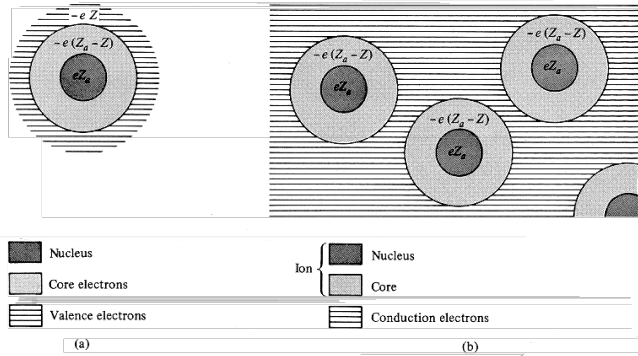
\includegraphics[scale=0.3]{ch1/image1.png}
	\captionof{figure}{Métal dans le modèle de Drude}
	\end{wrapfigure}
	\noindent
	\textbf{	Inclure tableau slide}
	Dans ce tableau, on peut voir $Z$ comme la valence, c'est à dire le nombre d'
	électrons qui vont jouer dans le conduction\footnote{Ne pas confondre avec $Z_a$, 
	le numéro atomique. On a donc $Z_a-Z$ électrons restant liés aux noyaux.}. La 
	densité du gaz d'électron de valence, donnant le nombre d'électrons par volume, 
	s'exprime 
	\begin{equation}
	n = N_A * \dfrac{Z\rho_m}{A} \approx 10^{22}\ \frac{e^-}{cm^3}
	\end{equation}
	où $N_A$ est le nombre d’Avogadro, $\rho_m$ la masse spécifique du matériau 
	([g/cm$^3$]) et $A$ la masse atomique de l'élément.
	
	\noindent
	Pour représenter cette densité, on utilise le paramètre $ r_s = \frac{r_0}{a_0}$
	où $a_0$ est le rayon de Bohr \footnote{$a_0 = 4 \pi \epsilon_0 \frac{\hbar^2}{m_e e^2}$}
	et $r_0$ le rayon d'une sphère contenant un seul 
	électron. On a alors : 
	\begin{equation}
	V_{sphère} = \frac{4\pi r^3_0}{3} = \text{Volume d'un électron} = \frac{1 e^-}{n} 
	\Longrightarrow r_0 = \left(\frac{3}{4\pi n}\right)^{1/3} \Longleftrightarrow r_s 
	= \left(\frac{3}{4\pi n a_0^3}\right)^{1/3}
	\end{equation}
	Ce paramètre est compris entre 2 et 3 pour la majorité des métaux et entre 3 et 6 
	pour les métaux alcalins.
	
\newpage
\section{Hypothèses de base du modèle de Drude}
Pour parvenir à son modèle, Drude émit quatre hypothèses

\begin{enumerate}
\item 
On postule l'\textit{
approximation des électrons indépendants} qui consiste à négliger l'interaction 
entre les électrons et l'\textit{approximations des électrons libre} qui consiste 
à négliger les interactions ion-électron. La première approximation est très
 pertinente mais la deuxième est à abandonner pour une compréhension qualitative du
 comportement des métaux. Ces approximations permettent de considérer que les électrons
 suivent un mouvemment "classique" (MRU en l'absence de champ extérieur, etc...).

\item Collisions instantanées : la vitesse d'un électron change brusquement 
lors d'une collision avec un cœur ionique.
		
\item C'est l'ingrédient phénoménologique : la probabilité de collision par unité de temps 
$1/\tau$ ([$s^{-1}$]) où $\tau$ est le temps de relaxation, que l'on suppose 
indépendant de la position et de la vitesse de l'électron\footnote{La probabilité 
de subir une collision sur un intervalle de temps $dt$ est $dt/\tau$.}.

\item Les collisions amènent à un équilibre thermodynamque local
 (après un nombre conséquent de collision, une seule ne suffit pas).
 Immédiatement après une collision, l'électron a une direction aléatoire et une 
 vitesse donnée par la distribution de la théorie cinétique des gaz.
\end{enumerate}


\section{Conductivité électrique "en courant continu" d'un métal}
On peut écrire la loi d'Ohm locale \footnote{ou bien $\vec(E) = \rho vec(j)$} 
\begin{equation}
\vec{j} = \sigma\vec{E}
\end{equation}
où $\sigma$ est le conductivité électrique et $\vec{j}$ est le vecteur densité de 
courant, la densité de charge qui traverse une surface unitaire par unité de temps.\\

Soit $n$ électrons par unité de volume se déplaçant à vitesse moyenne $\vec{v}$. Sur 
$dt$, ils parcourent $vdt$ et donc $n(vdt)S$ électrons vont traverser une surface $S$ 
perpendiculaire au courant. La charge électrique traversant la surface sera $-envdtS$.
Comme $I = dQ/dt$, on a $I = -nevS$. Par définition, $J = I/S$. La densité de courant 
vaut alors
\begin{equation}
\vec j = -e.n.S.\vec v\frac{1}{S} = -ne\vec{v}
\end{equation}

On va montrer que le temps entre deux collisions est le temps de relaxation. En $t=0$ 
la vitesse est $\vec{v_0}$ et immédiatement après une collision\footnote{$f = ma = eE 
\Leftrightarrow a = \frac{eE}{m} \Leftrightarrow v = \frac{eE\tau }{m}$} plus $-e\vec{E}
\tau/m$. Par l'hypothèse 4, $\vec{v_0}$ ne contribue pas à la vitesse moyenne :
\begin{equation}
\vec{v}_{moy} = \dfrac{-e\tau\vec E}{m}
\end{equation}
Avec la définition de $\vec j$, on obtient
\begin{equation}
\vec j = \dfrac{ne^2\tau}{m}\vec{E}
\end{equation}
En en déduit avec la loi d'Ohm locale que\\
\

\retenir{
\begin{equation}
\sigma = \dfrac{ne^2\tau}{m}
\end{equation}}
\newpage\noindent
Le \textbf{tableau} donne des temps de relaxations $\tau$ calculés par Drude. A noter 
que son odre de grandeur est $\approx\ 10^{-14}\ s$, ce que Drude avait conclut comme 
correct.  Hélas, la vitesse qu'il a considérée était fausse\footnote{Car la distribution 
d'un métal n'est pas maxwellienne}. La vitesse exacte donne lieu à des distances 
plus grandes qui peuvent encore s’agrandir à basse température : l’hypothèse des 
collision avec les cœur ionique est donc fausse, mais on peut utiliser ce modèle sans 
nous poser la question de la cause des collisions.

\section{Effet Hall et magnétorésistance}
Considérons un champ électrique $E_x$ selon $x$ appliqué au fil avec, en plus, un 
champ magnétique $\vec{H}$\footnote{C'est bien $\vec{H}$ le champ magnétique et non 
$\vec B$ qui est la densité de champ d'induction magnétique ! Biot et Savart permet 
en réalité de calculer $\vec{H}$ mais pas $\vec{B}$ (erreur fréquente). Cependant, 
seul $\vec{B}$ est mesurable, $\vec{H}$ "n'existe pas".} dirigé selon $z$. La force 
de Lorentz exercée sur les $e^-$ vaut 
\begin{equation}
-ev_x\vec{1_x}\times B\vec{1_z}
\end{equation}
Les électrons seront défléchis dans le sens $-y$ et un champ électrique $E_y$ va 
s'installer, dirigé vers les $y$ négatifs\footnote{Attention, la vitesse des 
électrons est bien opposée à celle de $\vec{j}$}. Ce champ à l'équilibre va 
contrebalancer la force de Lorentz : $|E_y| = |v_x|B$.\\

Deux grandeurs sont remarquables :
\begin{enumerate}
\item Remarquons la résistivité selon l'axe $x$ :
\begin{equation}
\rho(B) = \dfrac{E_x}{j_x}
\end{equation}
C'est la \textit{magnétorésistance\footnote{La magnétorésistance est la propriété 
qu'ont certains matériaux de présenter une résistance qui évolue lorsqu'ils sont 
soumis à un champ magnétique.} transverse} (car le champ magnétique est 
perpendiculaire au champ électrique), indépendante de $B$.

\item Le champ électrique transversal $E_y \propto B, j_x$. On définit le 
coefficient (ou constante) de Hall :
\begin{equation}
R_H = \dfrac{E_y}{j_xB}
\end{equation}
\end{enumerate}

	\begin{wrapfigure}[11]{l}{6.2cm}
	\vspace{-1cm}
	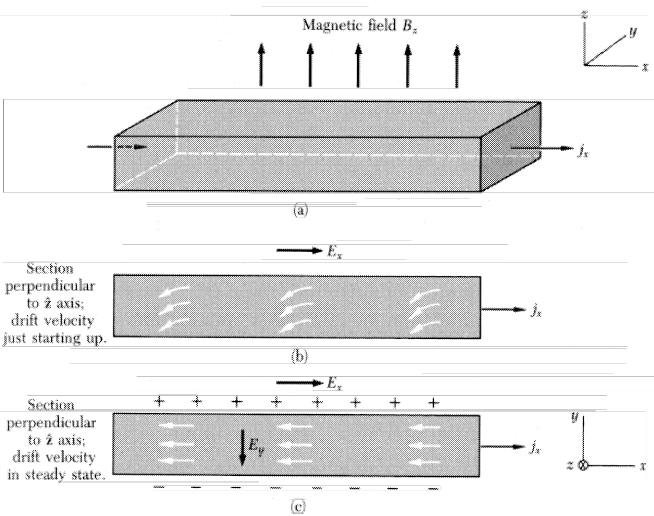
\includegraphics[scale=0.25]{ch1/image2.png}
	\captionof{figure}{Expérience de Hall}
	\end{wrapfigure}
Le signe de $j_x$ est indépendant du signe des porteurs de charge ainsi que de la force
de Lorentz. Si les charges sont positives, $E_y$ et $R_H$ seront positifs. On peut 
calculer ce coefficient :
\begin{equation}
-eE_y = ev_xB \Leftrightarrow -neE_y = nev_xB = j_xB \Longrightarrow R_H = -\frac{1}{ne}
\end{equation}
où $R_H$ est négatif car le champ de Hall est en -$\vec{1_y}$.